\subsection{Readability}\label{subsec:readability}

\subsubsection{Graph Layout}
% missing from graph paper
The Sugiyama Layout algorithm discussed in \cref{subsec:graphlayout} served the purpose of increasing visual clarity and readability of the TA outputted by TREAT.
Two of the most prevalent ways this was achieved was by layering the TAs states based on the length of the longest path from the initial state. The other was by ordering the states in each layer to achieve the smallest number of edge crossings.
While some of the specific approaches described by Mazetti et al. \cite{Mazetti2012} was not implemented into TREAT, the resulting implementation still greatly increases readability.

As mentioned in \cref{subsec:graphlayout}, the last step of the Sugiyama framework was not implemented, namely, properly positioning states in relation to each other. This might be developed in the future.

Another feature that would unequivocally improve readability is to visually separate transitions that share states, such as reversible transitions.
In all TAs pictured in \cref{subsec:graphlayout} and this section, any such transitions have been manually separated, since this feature has not been implemented. The difference can be seen on \cref{fig:transitions}.

\begin{center}
    \usetikzlibrary {automata,positioning}
\scalebox{0.9}{
    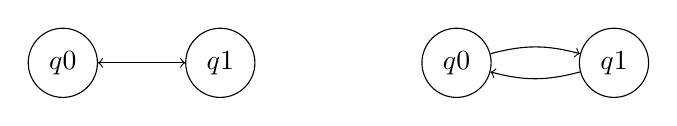
\begin{tikzpicture}[auto]
        \node[state] at (0, 0)(q0){$q0$};
        \node[state] at (2, 0)(q1){$q1$};
        \node[state] at (5, 0)(q2){$q0$};
        \node[state] at (7, 0)(q3){$q1$};

        \path[->]
        (q0)edge (q1)
        (q1)edge (q0)
        (q2)edge [bend left=15] (q3)
        (q3)edge [bend left=15] (q2)
        ;
    \end{tikzpicture}
}
\vspace{-1em}
\captionof{figure}{Comparison between implementation(Left) and intended behaviour(Right)}
\label{fig:transitions}
\end{center}

% formats
As described in \cref{output formats}, two output formats can be used to represent TAs.
The first format is UPPAAL. In UPPAAL, if no positions are given, the states are simply placed in a grid. This means, that using a graph layout algorithm is not strictly necessary.
To show its advantages, however, \cref{fig:treatLayout} shows the TA described in \cref{subsec:graphlayout}, which uses TREATs positioning, while \cref{fig:uppaalLayout} shows UPPAALs positioning. Both of these figures are constructed in UPPAAL

\begin{center}
    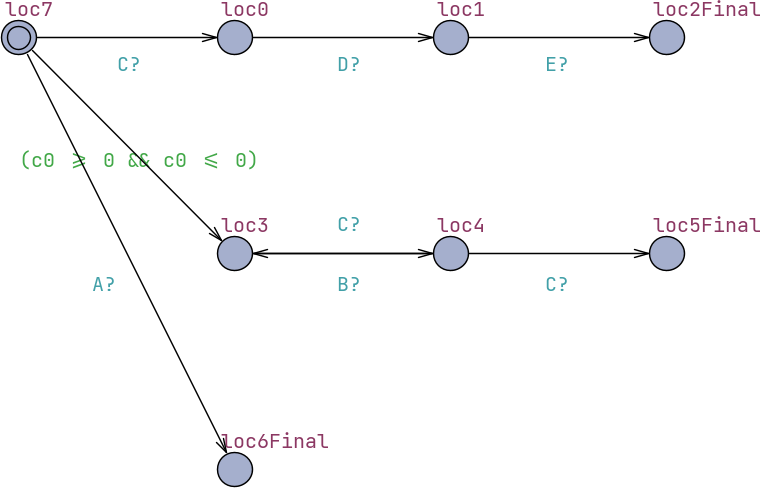
\includegraphics[width=0.8\columnwidth]{Documents/Diagrams/ReadabilityFigures/treat.png}
    \captionof{figure}{TA with TREATs state positioning.}
    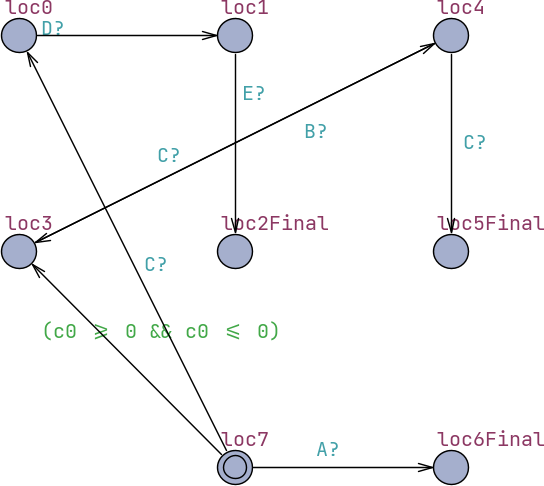
\includegraphics[width=0.6\columnwidth]{Documents/Diagrams/ReadabilityFigures/uppaal.png}
    \captionof{figure}{TA with UPPAALs state positioning.}
\end{center}
\vspace{1em}

The other output format is TikZ, used to represent graphs in LaTeX. Unlike UPPAAL, states in TikZ need positions, which necessitates some form of graph layout algorithm.

\subsubsection{Pruning}

The pruning steps described in \cref{sec:pruning} have an arguably greater effect to readability, since this can dramatically reduce the size and complexity of the output TA, while having no effect on the language accepted by the TA.
The TA on \cref{fig:nopruning} represents the same TRE as the one on \cref{fig:graph_step4}, except, no unreachable states, dead states, or dead transitions have been pruned.

\begin{center}
    \usetikzlibrary {automata,positioning}
% "(CDE|(BC)+)|A"
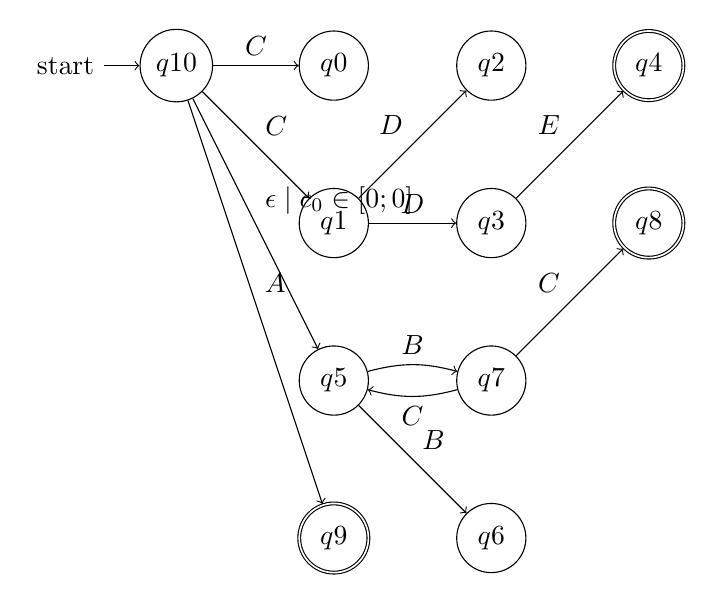
\begin{tikzpicture}[auto]
    \node[state] at (2, 0)(q0){$q0$};
    \node[state] at (2, -2)(q1){$q1$};
    \node[state] at (4, 0)(q2){$q2$};
    \node[state] at (4, -2)(q3){$q3$};
    \node[state, accepting] at (6, 0)(q4){$q4$};
    \node[state] at (2, -4)(q5){$q5$};
    \node[state] at (4, -6)(q6){$q6$};
    \node[state] at (4, -4)(q7){$q7$};
    \node[state, accepting] at (6, -2)(q8){$q8$};
    \node[state, accepting] at (2, -6)(q9){$q9$};
    \node[state, initial] at (0, 0)(q10){$q10$};

    \path[->]
    (q1)edge node{$D$}(q2)
    (q3)edge node{$E$}(q4)
    (q1)edge node{$D$}(q3)
    (q5)edge node{$B$}(q6)
    (q7)edge node{$C$}(q8)
    (q5)edge [bend left=15] node{$B$}(q7)
    (q7)edge [bend left=15] node{$C$}(q5)
    (q10)edge node{$C$}(q0)
    (q10)edge node{$C$}(q1)
    (q10)edge node{$\epsilon\mid c_0\in[0;0]$}(q5)
    (q10)edge node{$A$}(q9)
    ;
\end{tikzpicture}
\captionof{figure}{Graph layout with all pruning disabled.}
\label{fig:nopruning}
\end{center}
% maybe this figure is too big to include in the paper?

While disabling pruning on this example TA has significantly lowered the visual clarity, the TRE it represents is quite simple, and more complex TREs would only worsen the effect. This shows that pruning is a necessary step to ensure readability and visual clarity.